\documentclass[11pt]{article}

% -- Reduce PDF object streams & compression (mejora compatibilidad con PDF.js) --
\makeatletter
% Para pdfTeX (pdflatex)
\ifdefined\pdfobjcompresslevel
  \pdfobjcompresslevel=0 % deshabilita object streams
\fi
\ifdefined\pdfcompresslevel
  \pdfcompresslevel=0    % reduce/disable compresión de streams
\fi
\ifdefined\pdfminorversion
  \pdfminorversion=4     % forzar PDF 1.4 (opcional, mejora compatibilidad)
\fi
% Para LuaTeX / LuaLaTeX
\ifdefined\pdfvariable
  \pdfvariable objcompresslevel=0
  \pdfvariable compresslevel=0
\fi
\makeatother
% -----------------------------------------------------------------------


\input{../utils/preamble_problemas}
\usetikzlibrary{arrows.meta}

\title{Cálculo avanzado}
\author{Dpto. de Ingenería Mecánica}


\begin{document}
% \maketitle

\begin{center}
	\framebox[1.0\textwidth][c]{
		\huge{\textsc{Cálculo Avanzado}}
	}
\end{center}

\begin{center}
	\vspace{\baselineskip}
	\Large{\textsc{Departamento de Ingenería Mecánica}} \\
	\textsc{Facultad Regional La Plata} \\
	\textsc{Universidad Tecnológica Nacional}
\end{center}

% \vspace{1em}

\begin{center}
	\begin{tabular}{r l}
		\textbf{Práctica:}            & Unidad 8.                        \\
		\textbf{Tema:}                & Sistemas de ecuaciones lineales. \\
		\textbf{Profesor Titular:}    & Manuel Carlevaro.                \\
		\textbf{Ayudante de Primera:} & Christian Molina.                \\
	\end{tabular}\end{center}

\vspace{1em}

\begin{question} % Bradie Problemas 1-5 pg 171
	Escriba la matriz aumentada para los siguientes sistemas lineales de ecuaciones, y obtenga la solución usando eliminación gaussiana con sustitución hacia atrás:
	\begin{enumerate}[a)]
		\item \[ \begin{cases}2 x_1 - x_2 + x_3 = -1  \\
				      4 x_1 + 2 x_2 + x_3 = 4 \\
				      6 x_1 - 4 x_2 + 2 x_3 = -2
			      \end{cases} \]
		\item \[ \begin{cases}x_1 + 2 x_2 - x_3 = 1 \\
				      2 x_1 - x_2 + x_3 = 3 \\
				      -x_1 + 2 x_2 + 3 x_3 = 7
			      \end{cases} \]
		\item \[ \begin{cases}x_2 + x_3 + x_4 = 0         \\
				      3 x_1 + 3 x_3 - 4 x_4 = 7   \\
				      x_1 + x_2 + x_3 + 2 x_4 = 6 \\
				      2 x_1 - 3 x_2 + x_3 + 3 x_4 = 6
			      \end{cases} \]
	\end{enumerate}
\end{question}


\begin{question} % Bradie Problemas 10 pg 172
	\begin{enumerate}[a)]
		\item Resuelva el sistema:
		      \[ \begin{cases}
				      3.02 x_1 - 1.05 x_2 + 2.53 x_3 = -1.61 \\
				      4.33 x_1 + 0.56 x_2 - 1.78 x_3 = 7.23  \\
				      -0.83 x_1 - 0.54 x_2 + 1.47 x_3 = -3.38
			      \end{cases} \]
		      utilizando eliminación gaussiana con sustitución hacia atrás.
		\item Cambie el coeficiente de $x_1$ en la primera ecuación a $3.01$ y resuelva el sistema resultante. ¿En qué porcentaje cambian las componentes del nuevo vector solución?
		\item Vuelva el coeficiente de $x_1$ a su valor original en la primera ecuación, pero cambie el término independiente de la segunda ecuación a $1.99$ y resuelva el nuevo sistema. ¿Cuál es el cambio porcentual en las tres componentes de la solución comparados con sus valores de la parte a)?
	\end{enumerate}
\end{question}

\begin{question} % Bradie pg 206
	Verifique que las matrices triangulares $\mathbb{L}$ y $\mathbb{U}$ siguientes:
	\[ \mathbb{L} = \begin{bmatrix} 1 & 0 & 0 \\ 2 & 1 & 0 \\ 5 & 12 & 1 \end{bmatrix}, \quad \mathbb{U} = \begin{bmatrix} 1 & 4 & 3 \\ 0 & -1 & 3 \\ 0 & 0 & -53 \end{bmatrix} \]
	factorizan la matriz
	\[ \mathbb{A} = \begin{bmatrix} 1 & 4 & 3 \\ 2 & 7 & 9 \\ 5 & 8 & -2 \end{bmatrix} \]
\end{question}

\begin{question} % Bradie Ejercicio 11 pg 217
	Resuelva el sistema $\mathbb{A} \bm{x} = \bm{b}$ para cada uno de los siguientes términos independientes:
	\[ \mathbb{A} = \begin{bmatrix} 1 & 2 & 3 & 4 \\ -1 & 1 & 2 & 3 \\ 1 & -1 & 1 & 2 \\ -1 & 1 & -1 & 5 \end{bmatrix}, \, \bm{b}_1 = \begin{bmatrix} 10 \\ 5 \\ 3 \\ 4 \end{bmatrix}, \, \bm{b}_2 = \begin{bmatrix} -4 \\ -5 \\ -3 \\ -4 \end{bmatrix}, \, \bm{b}_3 = \begin{bmatrix} -2 \\ -3 \\ 1 \\ -8 \end{bmatrix} \]
\end{question}

\begin{question} % Burden Ejemplo 3 pg 295
	Resuelva el sistema lineal con aritmética de redondeo de tres dígitos y utilice una estrategia de pivoteo parcial escalado.
	\[ \begin{cases}
			2.11 x_1 - 4.21 x_2 + 0.921 x_3 + 2.01 \\
			4.01 x_1 + 10.2 x_2 - 1.12 x_3 = -3.09 \\
			1.09 x_1 + 0.987 x_2 + 0.832 x_3 = 4.21
		\end{cases} \]
\end{question}

\begin{question}
	Dado el siguiente sistema de ecuaciones:
	\[ \begin{system}
			2 x_1 + 5 x_2 + x_3 + 8 x_4 = 78 \\
			7 x_1 + 2 x_3 + x_4 = 24 \\
			x_1 + 4 x_2 + x_3 + 4 x_4 = 46 \\
			8 x_1 + 3 x_2 + 2 x_3 + 5 x_4 = 62
		\end{system} \]
	resolver el sistema implementando el método de Jacobi y el de Gauss-Seidel, con relajación, y comparar las velocidades de convergencia de cada método.
\end{question}

\begin{question} % Armadura - ejemplo de motivación, unidad 8
	Se desea analizar la armadura estáticamente determinada de la figura, con nodos
	$A=(0,0)$ m (apoyo fijo), $B=(2,0)$ m, $C=(4,0)$ m (apoyo móvil) y $D=(2, 1.6)$ m,
	sometida a una carga vertical $F = 10$ kN aplicada en $D$.

	\begin{center}
    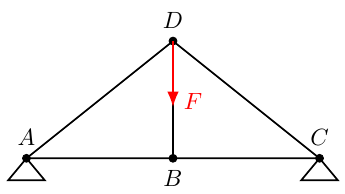
\includegraphics{figs/estructura.png}
		% \begin{tikzpicture}[
		% 		node/.style={circle, draw, fill=black, inner sep=1.3pt},
		% 		bar/.style={thick},
		% 		support/.style={thick},
		% 		force/.style={-{Latex[length=2.5mm]}, thick, red},
		% 		scale=1.2]
		% 	\coordinate (A) at (0,0);
		% 	\coordinate (B) at (2,0);
		% 	\coordinate (C) at (4,0);
		% 	\coordinate (D) at (2,1.6);
		%
		% 	\draw[bar] (A) -- (B) -- (C) -- (D) -- (A);
		% 	\draw[bar] (B) -- (D);
		%
		% 	\draw[support] (A) ++(-0.25,-0.3) -- ++(0.5,0) -- (A) -- cycle;
		% 	\draw[support] (C) ++(-0.25,-0.3) -- ++(0.5,0) -- (C) -- cycle;
		%
		% 	\foreach \p in {A,B,C,D}{\node[node] at (\p) {};}
		%
		% 	\draw[force] (D) -- ++(0,-0.9) node[below right, xshift=1pt, yshift=10.5pt] {$F$};
		% 	% \draw[force] (D) -- ++(0,-0.9) node[below right] {$F$};
		%
		% 	\node[above=2pt of A] {$A$};
		% 	\node[below=2pt of B] {$B$};
		% 	\node[above=2pt of C] {$C$};
		% 	\node[above=2pt of D] {$D$}; 
		% \end{tikzpicture}
	\end{center}

	La armadura tiene 5 barras ($AB$, $BC$, $AD$, $CD$, $BD$) y 3 reacciones de apoyo
	($A_x$, $A_y$, $C_y$). Planteando el equilibrio de fuerzas horizontal y vertical en
	cada uno de los 4 nodos se obtienen 8 ecuaciones lineales para las 8 incógnitas
	$\bm{x} = (A_x, A_y, N_{AB}, N_{BD}, N_{BC}, C_y, N_{AD}, N_{CD})^T$, donde $N_{ij}$
	es el esfuerzo normal en la barra $ij$ (positivo en tracción), que puede escribirse
	en la forma $\mathbb{A} \bm{x} = \bm{b}$.

	\begin{enumerate}[a)]
		\item Plantee las ecuaciones de equilibrio en los cuatro nodos ($A$, $B$, $C$ y
		      $D$) y arme la matriz $\mathbb{A}$ y el vector $\bm{b}$ del sistema.
		\item Resuelva el sistema por descomposición LU y obtenga las reacciones de
		      apoyo y el esfuerzo en cada barra, indicando si trabaja en tracción o
		      compresión.
		\item Intente resolver el mismo sistema con los métodos de Jacobi y de
		      Gauss-Seidel sin relajación ($\omega = 1$), partiendo de $\bm{x}^{(0)} = \bm{0}$.
		      Verifique que ninguno de los dos converge a la solución hallada en b) y
		      explique esta situación en términos de la dominancia diagonal de
		      $\mathbb{A}$.
		\item Aplique el método de sobrerrelajación sucesiva (SOR) visto en clase,
		      explorando valores de $\omega \in (0,2)$, y determine numéricamente el valor
		      de $\omega$ que minimiza el número de iteraciones necesarias para alcanzar
		      $\norm{\bm{x}^{(k)} - \bm{x}^{(k-1)}} < 10^{-8}$.
		\item Compare el desempeño de los tres enfoques (LU, Jacobi/Gauss-Seidel sin
		      relajar y SOR óptimo) en términos de tiempo de cómputo, número de
		      iteraciones y precisión alcanzada, y discuta en qué tipo de problemas de
		      ingeniería (p.\ ej.\ sistemas de gran escala provenientes del método de
		      elementos finitos) resulta preferible cada método.
	\end{enumerate}
\end{question}

\end{document}
